% =====================================================================
%  Chapter 5 — The Prior Art and the White Space
% =====================================================================

\chapter{The Prior Art and the White Space}
\label{ch:prior-art}

A book that builds a machine-learning investment system owes the reader an
account of what has already been built. This chapter surveys the work
closest to the one in this book, states what each of them actually
demonstrates, and identifies the space that is genuinely unoccupied.

\section{The closest work: DBOT}

The nearest neighbour in the literature is DBOT, by Dhar and Sedoc, posted
as arXiv preprint 2504.05639 in April 2025 and registered with a DataCite
identifier of 10.48550/arXiv.2504.05639. The paper fine-tunes GPT-4o on
Damodaran's \emph{Musings on Markets} --- the collected valuation notes of
one of the most widely-read equity analysts alive --- and asks whether a
language model that has read a decade of professional thinking can be
made to produce systematic investment decisions.

The claim of the paper is about \emph{stability}, and it is a legitimate and
interesting claim. The authors show that the fine-tuned model produces
internally consistent, reproducible valuations, that its outputs are stable
under perturbation, and --- this is the part that matters for the
argument of this book --- that the resulting process is \emph{backtestable}.
That is, the paper's contribution is to remove the obstacle that had
prevented LLM-based investment systems from being evaluated at all: the
inconsistency that would have made any backtest of such a system
meaningless.

Read carefully, the paper reports no portfolio performance. There is no
return series, no equity curve, no Sharpe ratio, no drawdown, no comparison
with a benchmark, and no transaction-cost or tax treatment. The
demonstration is that a stable, evaluable system \emph{can} be built. The
evaluation itself is left as future work.

That is the white space this book occupies, and it is worth being precise
about the distinction, because the two artefacts are different in kind and
the difference is the subject of the book. DBOT demonstrates
\emph{evaluability}. This book demonstrates an \emph{evaluation}. The
first removes a barrier; the second walks through it and reports what is on
the other side, including the parts that are disappointing.

\section{The 2025--26 frontier}

Four items from the current frontier frame the problem.

\textbf{Signature-Informed Transformer for Asset Allocation} (arXiv
2510.03129) works with the path-dependent signature of the price process
rather than with a fixed-length return window, which addresses a real and
underrated weakness of window-based features: that the \emph{order} of
returns carries information that a summary statistic discards.

\textbf{DeePM} (arXiv 2601.05975, Oxford) is explicitly about regime
robustness in systematic macro portfolio management --- that is, about
making a learned allocator robust to the fact that the data generating
process changes. Its problem statement is the same one this book confronts
from the other side: rather than making the model robust to regime change
by clever architecture, this book makes the \emph{portfolio} robust to it
by refusing to let the model set the strategic allocation, and by shrinking
the model's contribution toward zero whenever the posterior over the edge
is indistinguishable from the null.

\textbf{A systematic review of reinforcement learning for automated equity
portfolio management} (published in \emph{Discover Computing} in 2026,
doi 10.1007/s10791-026-10336-1) surveys 156 articles published between 2018
and 2025. Its existence is itself a finding: the depth of the applied
literature is remarkable, and so is the fact that it needed a systematic
review to be legible at all.

\textbf{The empirical result inside that frontier} is the one that should
give a single investor pause. In a 2026 deep reinforcement learning study
for global equity portfolios, a recurrent network beat a Transformer
outright. The lesson is not that LSTM networks are superior to attention
mechanisms; the subject matter is too new and too narrow to support that.
The lesson is that a well-specified recurrent model can beat a
heavier architecture on a noisy target --- which is a statement about the
\emph{target}, not about the architecture. The target is noisy because the
signal is weak; no architecture fixes that.

\begin{figure}[!htbp]
\centering
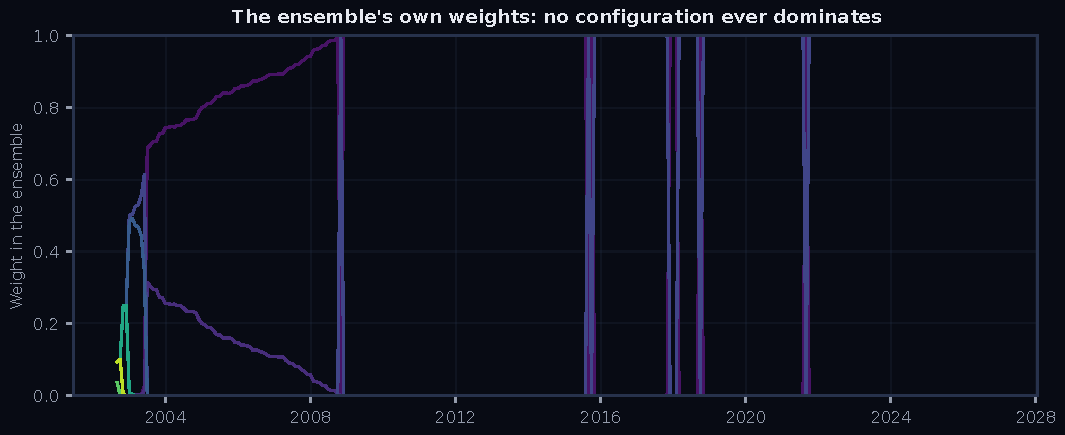
\includegraphics[width=\textwidth]{../figures/fig_model_weights.pdf}
\caption{The running model average. Each member of the ensemble carries a
weight that depends only on outcomes already realised at the formation
date. The weights are close to uniform for long stretches, which is itself
the finding: the members rarely disagree enough for the average to prefer
one strongly.}
\label{fig:model-weights}
\end{figure}

\section{Why the field's centre of gravity is in the wrong place for this reader}

Almost all of the literature above optimises for \emph{raw predictive
accuracy} or \emph{portfolio return}, on institutional or simulated
institutional data, with futures and options available, and with a
shorter horizon than this book concerns.

Three of those four differences are fatal to transferring the results to
this book's setting, and the fourth is not fatal but is important.

Options and futures are excluded here by the owner's scope: the universe is
equities and exchange-traded funds. That rules out the hedging overlays
that most of the deep reinforcement learning literature treats as
standard, and it changes the problem, because without derivatives the only
tools for reducing drawdown are cash, sector and factor tilts, and the
governor must work through exposure rather than through a hedge.

The horizon difference is the most consequential. A quarterly or monthly
trading objective with a Sharpe-based reward is a different problem from a
twenty-year one, and Chapter 8 shows that the difference is not academic:
the evaluation frequency itself changes the equity premium an investor
harvests, by an amount that is comparable to the entire premium.

The institutional setting matters because the capacity assumptions are
wrong in the reader's direction. A backtest that assumes frictionless
execution at mid-prices is not conservative for a single investor, who
faces the bid--ask spread on every one of perhaps two trades a month. It is
optimistic, and the difference is real.

\section{What is actually unoccupied}

Having surveyed, the unoccupied space is fourfold, and each part is
occupied by this book.

\begin{enumerate}
\item \textbf{An evaluated system, not an evaluable one.} The frontier
demonstrates that machine-learning allocators can be built and made stable.
The literature surveyed in Chapter 3 and the review article above do not
supply a fully specified system whose out-of-sample performance, net of
costs and taxes, has been measured against a stated benchmark with a
declared trial family.
\item \textbf{The individual's constraint set.} Not capacity, not market
impact, not the institutional tax treatment. Bid--ask spread, the wash-sale
rule, the \$3,000 capital-loss offset, the one-year holding period, and the
behavioural failure modes of one person trading their own money.
\item \textbf{A selection-corrected verdict.} The evaluation machinery of
Part IV is not applied to somebody else's strategy; it is applied to the
system in this book, whose full family of tried configurations is
enumerated in the text.
\item \textbf{An honest null.} The book is written so that the result
``the machine adds essentially nothing over the stated allocation and the
risk governor'' is a publishable, coherent, and useful finding --- because
that is what the measurements show, and because a book that reports a null
result with the same rigour as an alpha is more useful than one that
reports only alphas.
\end{enumerate}

\begin{takeaway}[The white space]
The prior art establishes that machine-learning investment systems can be
built and made stable enough to backtest. It does not supply an end-to-end
evaluation of such a system for an individual investor, net of costs and
taxes, with the trial family declared. That is the gap, and it is where
this book works.
\end{takeaway}

\begin{keytakeaways}
\item DBOT (arXiv 2504.05639) establishes that a language-model investment
process can be made stable enough to backtest; it reports no portfolio
performance at all.
\item The 2025--26 frontier is deep and largely institutional, and a
recurrent model beating a Transformer on a noisy target is evidence about
the target, not the architecture.
\item The four gaps are the evaluated system, the individual's constraint
set, the selection-corrected verdict, and an honest null.
\end{keytakeaways}
